% 1405/8/19
% H. Behrouz 
% Email : Texlivegroup@gmail.com



\documentclass[a4paper]{book}
\usepackage[paperwidth=15.1cm,paperheight=22.1cm,inner=1.8cm,outer=1.5cm,top=2cm,bottom=2cm,includefoot]{geometry}

\usepackage{amsmath,amssymb,amsthm}
\usepackage{mathtools}
\usepackage{graphicx}
\usepackage{geometry}
\usepackage{fancyhdr}
\usepackage{titlesec}
\usepackage{titletoc}
\usepackage{hyperref}
\usepackage{xcolor}
\usepackage{setspace}
\usepackage{booktabs}
\usepackage{enumitem}
\usepackage{listings}
\usepackage{appendix}
\usepackage{float}
\usepackage{tikz}
\usepackage{multicol}


\usepackage{xepersian}
\settextfont{XB Niloofar}
\setlatintextfont{XB Niloofar}
\setdigitfont{XB Niloofar}


% تنظیمات صفحه 
\geometry{
    top=2.5cm,
    bottom=2.5cm,
    left=3cm,
    right=2.5cm
}

% تنظیمات فونت و فاصله خطوط 
\onehalfspacing

% رنگ‌های لینک 
\hypersetup{
colorlinks=true,
linkcolor=blue,
citecolor=green,
urlcolor=magenta,
pdftitle={عنوان کتاب},
pdfauthor={نام نویسنده}
}

% تنظیمات سرصفحه و پاصفحه 
\pagestyle{fancy}
\fancyhf{}
\fancyhead[LE,RO]{\thepage}
\fancyhead[RE]{\leftmark}
\fancyhead[LO]{\rightmark}
\renewcommand{\headrulewidth}{0.4pt}

\fancypagestyle{plain}{
\fancyhf{}
\fancyfoot[C]{\thepage}
\renewcommand{\headrulewidth}{0pt}
}

% تنظیمات فصل و بخش 
\titleformat{\chapter}[display]
{\normalfont\huge\bfseries}
{\chaptertitlename\thechapter}{20pt}{\Huge}

\titlespacing*{\chapter}{0pt}{-30pt}{40pt}

% محیط‌های قضیه 
\newtheorem{theorem}{قضیه}[chapter]
\newtheorem{lemma}[theorem]{لم}
\newtheorem{corollary}[theorem]{نتیجه}
\newtheorem{definition}[theorem]{تعریف}
\newtheorem{example}[theorem]{مثال}

% اطلاعات کتاب ====================
\title{\Huge\textbf{عنوان کتاب شما}}
\author{\Large
 نام نویسنده 
\\[0.5cm] 
\small
 نام و نام خانوادگی
}
\date{
$19$
آبان
$1405$
}





\newcommand{\dicalphabet}[1]{
\begin{minipage}{\columnwidth}
\centerline{\noindent\textbf{\large #1 }}
\vspace{.5em}
\end{minipage}
\nopagebreak[4]
}
\newcommand{\dic}[2]{\noindent  #2 \dotfill  \lr{#1} \\ }
% ==================== شروع سند ====================
\begin{document}


% در زیر به جای Wallpaper می‌توانید عکس دلخواه برای صفحه تصویر انتخاب کنید
\begin{tikzpicture}[remember picture, overlay]
\node[inner sep=0pt] at (current page.center) {%
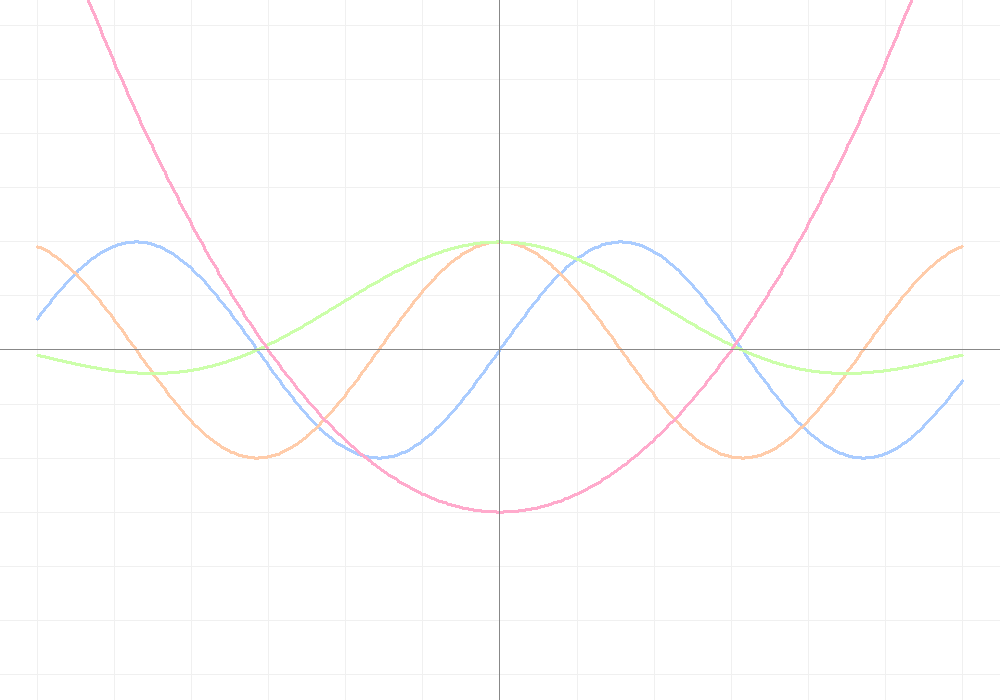
\includegraphics[width=\paperwidth,height=\paperheight]{Wallpaper}%
};%
\end{tikzpicture}

{\Huge 
\textcolor{red}{
\textbf{
عنوان کتاب
}
}
}
\\[1.5cm]
{{\Large 
\textcolor{red}{
\textbf{
نام نویسنده در صفحه تصویر
}
}
}}


\let\cleardoublepage=\clearpage




% ---------- صفحه عنوان ----------
\frontmatter
\maketitle

% ---------- تقدیم‌نامه ----------
\newpage
\thispagestyle{empty}
\vspace*{5cm}
\begin{center}
\textit{
تقدیم به ...
}
\end{center}

% ---------- پیش‌گفتار ----------
\chapter*{پیش‌گفتار}
\addcontentsline{toc}{chapter}{پیش‌گفتار}
متن پیش‌گفتار خود را اینجا بنویسید...


\let\cleardoublepage=\clearpage
% ---------- فهرست مطالب ----------
\tableofcontents

% ---------- فهرست اشکال ----------
\listoffigures

% ---------- فهرست جداول ----------
\listoftables

% متن اصلی 
\mainmatter

\chapter{مقدمه}
\label{ch:intro}

این فصل مقدمه‌ای بر موضوع کتاب است.

\section{پیشینه}
\label{sec:background}

متن بخش اول...


\subsection{زیربخش}
متن زیربخش...

\section{هدف کتاب}
هدف این کتاب بررسی... است.

\begin{definition}[تعریف نمونه]
\label{def:sample}
این یک تعریف نمونه است.
\end{definition}

\begin{theorem}
\label{thm:sample}
اگر $a$ و $b$ اعداد حقیقی باشند، آنگاه $a + b = b + a$.
\end{theorem}

\begin{proof}
اثبات بدیهی است.
\end{proof}

\begin{figure}[H]
 \centering
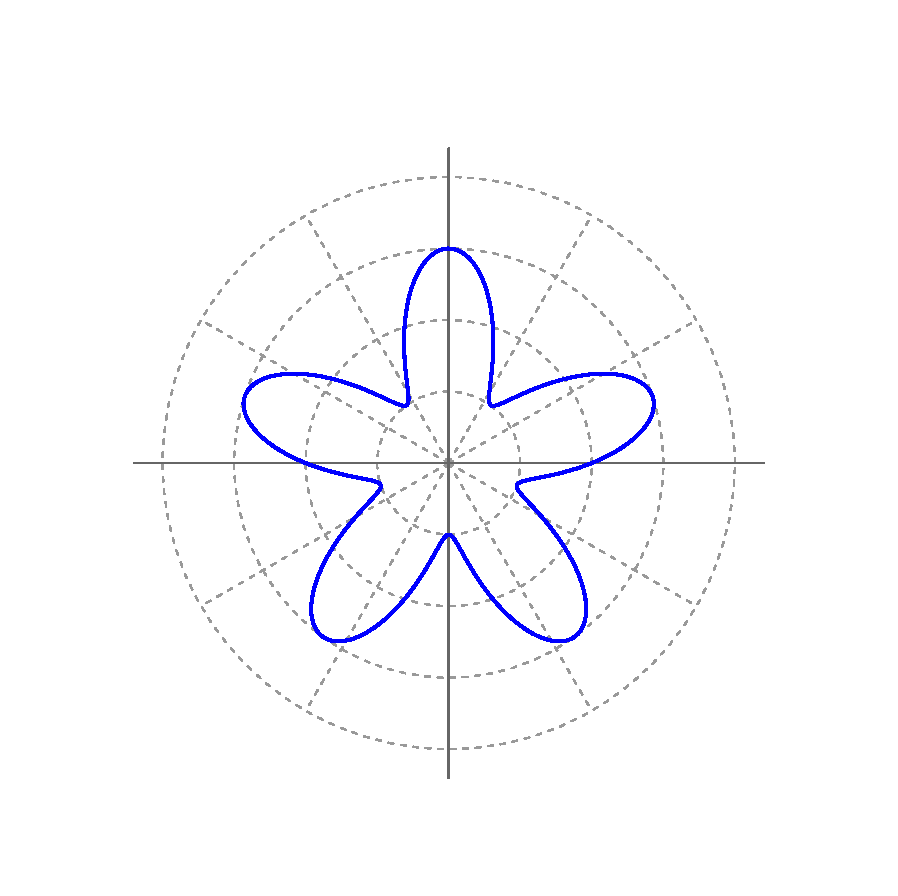
\includegraphics[width=0.7\textwidth]{f1}
\caption{نمونه شکل}
\label{f1}
\end{figure}

\begin{table}[H]
    \centering
    \caption{نمونه جدول}
    \label{tab:sample}
    \begin{tabular}{ccc}
        \toprule
        ستون ۱ & ستون ۲ & ستون ۳ \\
        \midrule
        ۱ & ۲ & ۳ \\
        ۴ & ۵ & ۶ \\
        \bottomrule
    \end{tabular}
\end{table}

\chapter{فصل دوم}
\label{ch:two}

متن فصل دوم...\label{ch:intro}

این فصل مقدمه‌ای بر موضوع کتاب است.

\section{پیشینه}
\label{sec:background}

متن بخش اول...

\subsection{زیربخش}
متن زیربخش...

\section{هدف کتاب}
هدف این کتاب بررسی... است.

\begin{definition}[تعریف نمونه]
\label{def:sample}
این یک تعریف نمونه است.
\end{definition}

\begin{theorem}
\label{thm:sample}
اگر $a$ و $b$ اعداد حقیقی باشند، آنگاه $a + b = b + a$.
\end{theorem}

\begin{proof}
اثبات بدیهی است.
\end{proof}

\begin{figure}[H]
 \centering
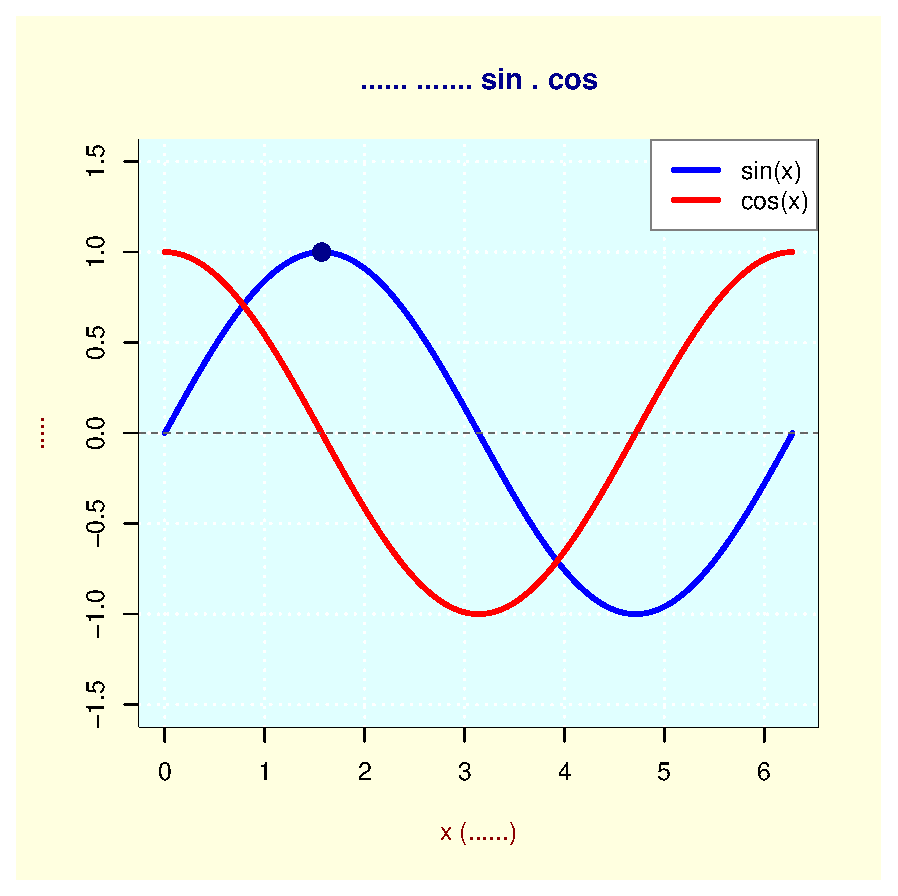
\includegraphics[width=0.6\textwidth]{f2}
\caption{نمونه شکل}
\label{f2}
\end{figure}

\begin{table}[H]
    \centering
    \caption{نمونه جدول}
    \label{tab:sample}
    \begin{tabular}{ccc}
        \toprule
        ستون ۱ & ستون ۲ & ستون ۳ \\
        \midrule
        ۱ & ۲ & ۳ \\
        ۴ & ۵ & ۶ \\
        \bottomrule
    \end{tabular}
\end{table}











% پیوست‌ها 
\appendix
\chapter*{پیوست}
\addcontentsline{toc}{chapter}{پیوست}
\markboth{پیوست}{پیوست}

محتوای پیوست...






% واژه‌نامه 






\chapter*{واژه‌نامه}
\addcontentsline{toc}{chapter}{واژه‌نامه}
\markboth{واژه‌نامه}{واژه‌نامه}

\begin{multicols}{2}
%\small

\dicalphabet{آ}
\dic{Axiom}{اصل موضوع}
\dic{Algorithm}{الگوریتم}
\dic{Integral}{انتگرال}
\dic{Ideal}{ایده‌آل}
\dic{Probability}{احتمال}
\dic{Identity}{اتحاد}

\dicalphabet{ب}
\dic{Eigenvector}{بردار ویژه}




\dicalphabet{پ}
\dic{Basis}{پایه}



\dicalphabet{ت}
\dic{Topology}{توپولوژی}
\dic{Bijection}{تابع دوسویی}
\dic{Transformation}{تبدیل}
\dic{Function}{تابع}


\dicalphabet{ح}
\dic{Limit}{حد}

\dicalphabet{خ}
\dic{Manifold}{خمینه}

\dicalphabet{د}
\dic{Determinant}{دترمینان}




\dicalphabet{ر}
\dic{Equivalence Relation}{رابطه هم‌ارزی}
\dic{Relation}{رابطه}

\dicalphabet{ش}
\dic{Lattice}{شبکه}

\dicalphabet{ف}
\dic{Metric Space}{فضای متری}
\dic{Vector Space}{فضای برداری}
\dic{Hilbert Space}{فضای هیلبرت}

\dicalphabet{ق}
\dic{Theorem}{قضیه}




\dicalphabet{گ}
\dic{Group}{گروه}
\dic{Abelian Group}{گروه آبلی}

\dicalphabet{م}
\dic{Matrix}{ماتریس}
\dic{Eigenvalue}{مقدار ویژه}
\dic{Field}{میدان}
\dic{Boundary}{مرز}
\dic{Derivative}{مشتق}
\dic{Differential Equation}{معادله دیفرانسیل}

\dicalphabet{ن}
\dic{Norm}{نُرم}
\dic{Mapping}{نگاشت}

\dicalphabet{ه}
\dic{Homomorphism}{همریختی}
\dic{Convergence}{همگرایی}






\dicalphabet{ی}
\dic{Isomorphism}{یک‌ریختی}


\end{multicols}








% منابع 
\addcontentsline{toc}{chapter}{کتاب‌نامه}

\begin{thebibliography}{9}
\begin{persian}

\bibitem{R1}
مرجع فارسی را وارد کنید ...
\bibitem{R2}
مرجع فارسی را وارد کنید ...

\end{persian}
\begin{latin}

\bibitem{R3} 
enter english bibliography ...

\bibitem{R4}
enter english bibliography ...


\end{latin}
\end{thebibliography}











\end{document}


